\subsection{Ampliación de palabra}
Para ampliar la palabra de una memoria, se debe agregar un chip de memoria adicional. Por ejemplo, si se tiene una memoria de $1k$ palabras de $8$ bits cada una y se desea ampliar la palabra a $16$ bits, se debe agregar un chip de memoria adicional.

\begin{figure}[h]
    \centering
    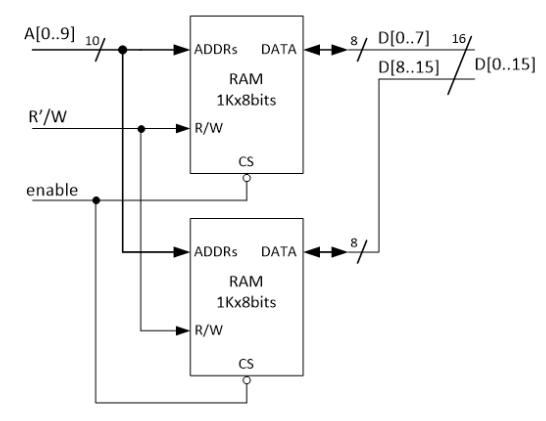
\includegraphics[scale=0.8]{img/memparalelo.png}
\end{figure}

En este ejemplo, las líneas de datos de D0 a D7 corresponden a la primera palabra de $8$ bits y las líneas de datos de D8 a D15 corresponden a la segunda palabra de $8$ bits, se juntan para formar una palabra de $16$ bits.